\documentclass{article}
\usepackage[utf8]{inputenc}
\usepackage{graphicx}
\usepackage{amsmath}
\usepackage{titling}
\usepackage{pdflscape}
\usepackage[export]{adjustbox}
\usepackage{float}
\usepackage{booktabs} % To thicken table lines
\usepackage{adjustbox}

\setlength{\droptitle}{-10em}
\pagestyle{empty}

\title{Lab. 4 - Clustering di dati medici}
\author{Ballarin Simone, Gobbo Alessio, Rossi Daniel}
\date{June 2019}

\begin{document}
\maketitle

\section*{Domanda 1}
Viene riportato il grafico ottenuto dall'esecuzione dell'algoritmo Gerarchico.\\
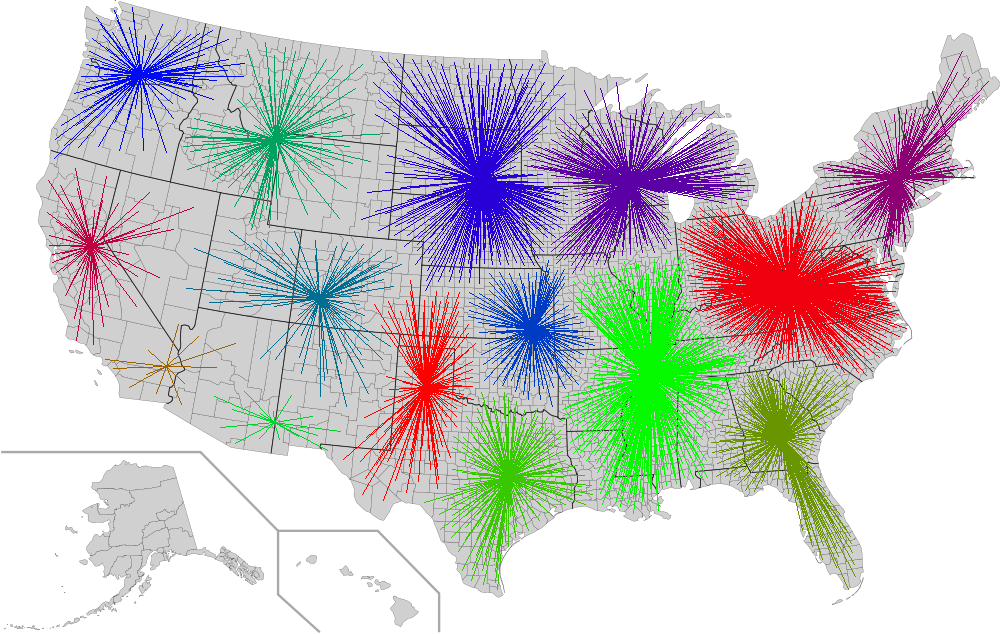
\includegraphics[width=1.0\linewidth, valign=t]{figures/Domanda1}

\section*{Domanda 2}
Viene riportato il grafico ottenuto dell'esecuzione dell'algoritmo Kmeans.\\
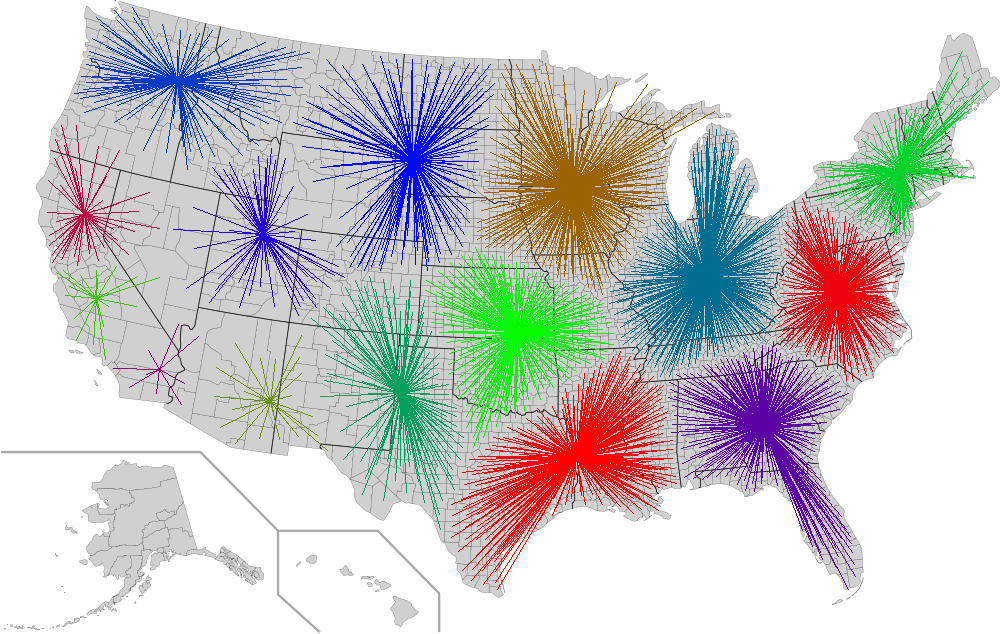
\includegraphics[width=1.0\linewidth, valign=t]{figures/Domanda2}

\section*{Domanda 3}
Dati $q$ il numero di iterazioni di \textit{kmeans}, $k$ il numero di clustering e $n$ la cardinalità dell'insieme dei punti, possiamo quantificare le seguenti complessità dei due algoritmi di clustering:
\begin{itemize}
\item La complessità del clustering gerarchico è $O(n\,h(n))$, dove $h(n)$ è la complessità della ricerca dei punti più vicini.
Questa ricerca è stata effettuata con la funzione \textit{FastestClosestPair}, la quale ha complessità $O(n\,log(n))$;
Quindi complessivamente il clustering gerarchico ha complessità $O(n^2\,log(n))$.
\item La complessità di \textit{kmeans} invece è di $O(q\,n\,k)$. 
\end{itemize}

\noindent Ipotizzando quindi $q$ e $k$ fattori molto piccoli, quindi trascurabili come segue $q \approx 1$ e $k \approx 1$, giungiamo alla conclusione che 
la complessità del clustering gerarchico rimanga inalterata, mentre \textit{kmeans} giunga a $O(n)$.\\
Da quando appena esposto risulta evidente come \textit{kmeans} sia in termini asintotici, e considerando $q$ e $k$ insignificanti, significativamente piu' efficienti.

\section*{Domanda 4}
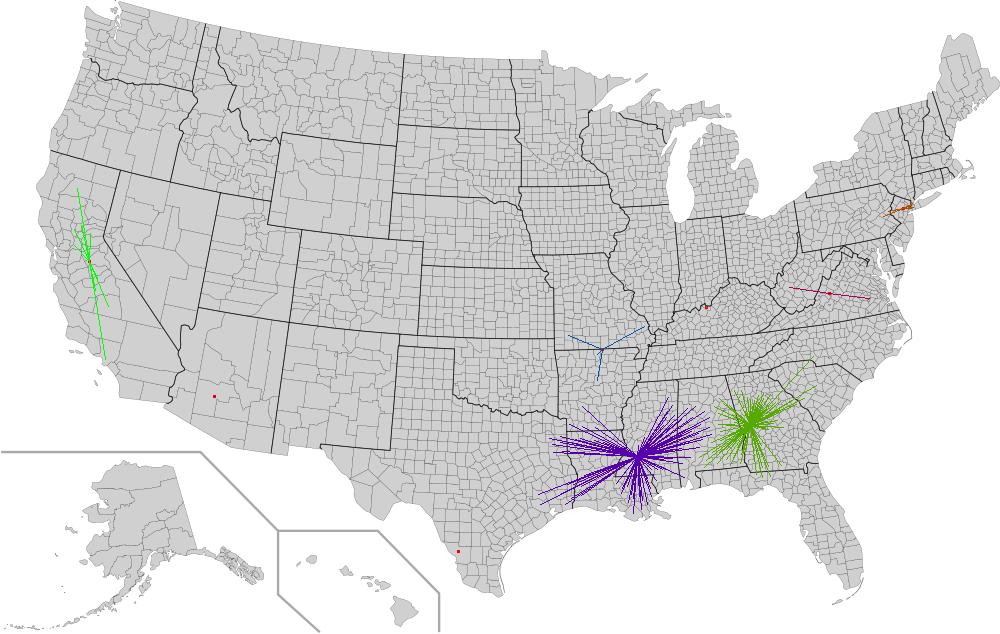
\includegraphics[width=1.0\linewidth, valign=t]{figures/Domanda4}

\section*{Domanda 5}
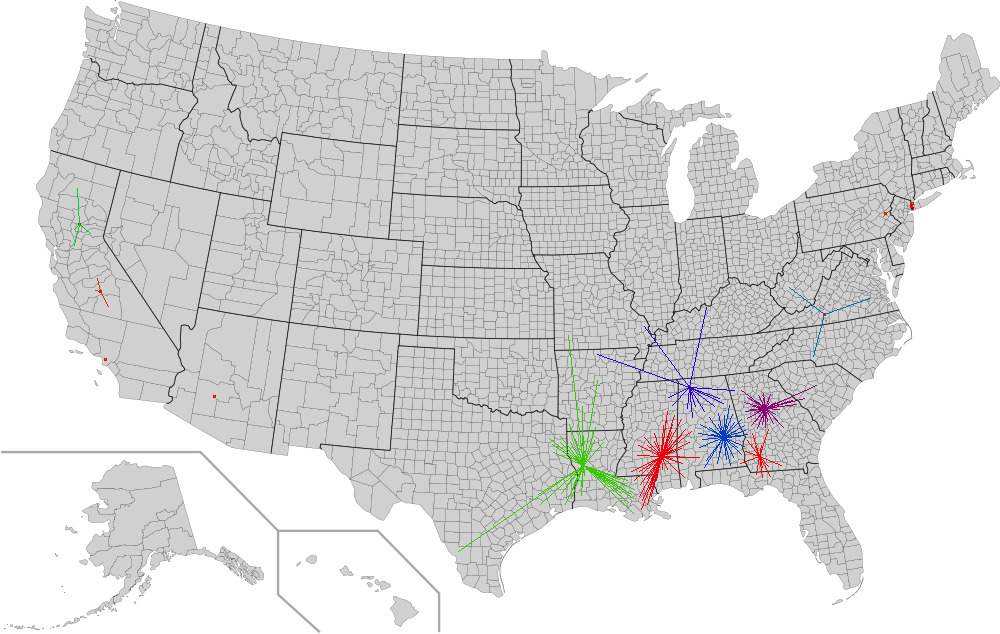
\includegraphics[width=1.0\linewidth, valign=t]{figures/Domanda5}

\end{document}